\chapter{На каких языках программирования пишутся операционные системы}
\label{ch:operating-sysmets}

В главе исследуется объект Викиданных <<операционная система>> (operating system) и его свойства. В каждом из разделов представлены задачи, решённые с помощью SPARQL-запросов. В их числе: нахождение экземпляров объекта <<операционная система>>, построение списков операционных систем (ОС) содержащих информацию о их <<предках>>\footnotemark,
\footnotetext{Операционных систем, послуживших основой для создания новой}
времени их создания, языков программирования, на котором написана ОС. Также построена гистограмма, показывающая количество программ, написанных на том или ином языке программирования, и какая доля из них работает под той или иной ОС. У большого количества операционных систем в Викиданных не указан язык программирования, на котором она разрабатывалась, а именно на 2020 год это свойство указано всего у 29\% из общего количества систем. Викиданные играют большую роль в документировании программного обеспечения. Но в то же время Викиданные стремительно заполняются и играют большую роль в документировании программного обеспечения.

\section{Список операционных систем}
Ниже представлен SPARQL-запрос для получения списка всех операционных систем (листинг \ref{lst:all_operating_systems}).

\begin{lstlisting}[ language=SPARQL, 
	caption={\href{https://w.wiki/n89}{Список всех опрационных систем}\protect\footnotemark},
	label=lst:all_operating_systems
	]
SELECT ?os ?osLabel
WHERE
{
	?os wdt:P31 wd:Q9135. # instance of operating system
SERVICE wikibase:label { bd:serviceParam wikibase:language "ru, en" }
}
\end{lstlisting}
\footnotetext{Получено \num{510} операционных систем в 2017 году, и \num{1086} в 2020 году.  Ссылка на SPARQL-запрос: \href{https://w.wiki/n89}{https://w.wiki/n89}}

Наиболее полными и проработанными операционными системами на Викиданных являются: \wdqName{Microsoft Windows}{1406} \wdqName{Windows 8}{5046}, \wdqName{GNU}{44571}, \wdqName{Windows 10}{18168774}, имеющие по 24 заполненных свойства\cite{prowd_os_link}.

Почти пустыми и малоинформативными операционными системами оказались: \wdqName{Novell DOS}{3345389}, \wdqName{MagiC}{1884068}, \wdqName{KallistiOS}{1722492}, и другие. У данных систем заполнено всего одно свойство\cite{prowd_os_link}.

По данным ProWD у единственной в Викиданных отечественной операционной системы \wdqName{Miraculix}{4044344} заполнено семь свойств\cite{prowd_os_link_ru}.

\section{Предшественники операционных систем}
В листинге \ref{lst:base_of_operating_systems} представлен SPARQL-запрос для получения списка \href{https://www.wikidata.org/wiki/Property_talk:P144}{базовых (P144)} операционных систем. Этот запрос показывает соответствие между \wdqName{операционной системой}{9135} и её <<предком>>, то есть предшествующей операционной системой, на котором она основана.

\marginnote{
	Выберите ОС, на основе какой из операционных систем
	\href{https://w.wiki/n8U}{Debian}, 
	\href{https://w.wiki/n8V}{Android}, 
	\href{https://w.wiki/n8W}{Ubuntu}, 
	\href{https://w.wiki/n8X}{ядро Linux} 
	было создано больше всего других операционных систем?\\
	См. ответ~\ref{answer:os_base} на с.~\pageref{answer:os_base}.
}

\begin{lstlisting}[ language=SPARQL, 
	caption={\href{https://w.wiki/v5K}{Список базовых операционных систем}\protect\footnotemark},
	label=lst:base_of_operating_systems
	]
SELECT ?os ?osLabel ?base ?baseLabel
WHERE
{
	?os wdt:P31 wd:Q9135. # is instance of operating system
	?os wdt:P144 ?base. # is based on ?base
SERVICE wikibase:label { bd:serviceParam wikibase:language "ru, en" }
}
\end{lstlisting}
\footnotetext{Получено \num{47} базовых операционных систем в 2017 году, и \num{118} в 2020 году. Ссылка на SPARQL-запрос: \href{https://w.wiki/v5K}{https://w.wiki/v5K}}

\section{Дата выпуска операционных систем}

В листинге \ref{lst:inception_time_of_operating_systems} представлен SPARQL-запрос для получения списка операционных систем с указанием даты их создания.

\marginnote{
	Какую из операционных систем
	\href{https://w.wiki/n8P}{Newton OS},
	\href{https://w.wiki/n8Q}{Ubuntu Touch} или
	\href{https://w.wiki/n8R}{JavaOS}
	разработала компания \href{https://w.wiki/n8S}{Apple}?
	
	См. ответ~\ref{answer:what_system_created} на с.~\pageref{answer:what_system_created}.
}

\index{SPARQL!hide!Список операционных систем с датой их создания}
\index{График!Timeline!Часть временной шкалы с датами выпуска операционных систем с 1955 по 2020 год}
\begin{lstlisting}[ language=SPARQL, 
	caption={\href{https://w.wiki/v5Z}{Список операционных систем с датой их создания}\protect\footnotemark},
	label=lst:inception_time_of_operating_systems
	]
#defaultView:Timeline{"hide": "?when"}
SELECT DISTINCT ?os ?osLabel ?when (YEAR(?when) as ?date) ?pic
WHERE
{
	?os wdt:P31 wd:Q9135. # instance of operating system
	?os wdt:P571 ?when. # inception date
	OPTIONAL { ?os wdt:P18 ?pic }
SERVICE wikibase:label {bd:serviceParam wikibase:language "ru, en"}
}
\end{lstlisting}
\footnotetext{Получено \num{30} дат создания в 2017 году, и \num{238} в 2020 году. Ссылка на SPARQL-запрос: \href{https://w.wiki/v5Z}{https://w.wiki/v5Z}}

При создании SPARQL-запроса \ref{lst:inception_time_of_operating_systems} использовалась опция \{"hide": "?when"\} для команды \#defaultView:Timeline\footnotemark.
\marginnote[0.5cm]{}
\footnotetext{Команда \#defaultView:Timeline, которая выглядит как комментарий, на самом деле является инструкцией Wikidata Query Service (кратко WDQS), чтобы результат был представлен не в виде таблицы(по умолчанию), а на временной шкале, см. рис. \ref{lst:count_os_on_languages}}
\marginnote[0.3cm]{}
Эта опция позволяет использовать данные для создания внешнего вида запроса, без их непосредственного отображения\cite{query_wiki}.

Листинг \ref{lst:inception_time_of_operating_systems} показывает в красивой графической оболочке (рисунок \ref{fig:os_creation}) временной шкалы (англ. timeline) создания (на самом деле выпуска\footnotemark) операционных систем. А также он показывает насколько плохо заполнены Викиданные, так как в запросах выводится только 230 операционных систем (это 21\% от всего количества) на 2020 год. Что, в свою очередь, означает, что у оставшихся объектов поле дата создания попросту не заполнено. Хотя информация о дате выпуска не такая уж и секретная.

\begin{figure*}[h!]
	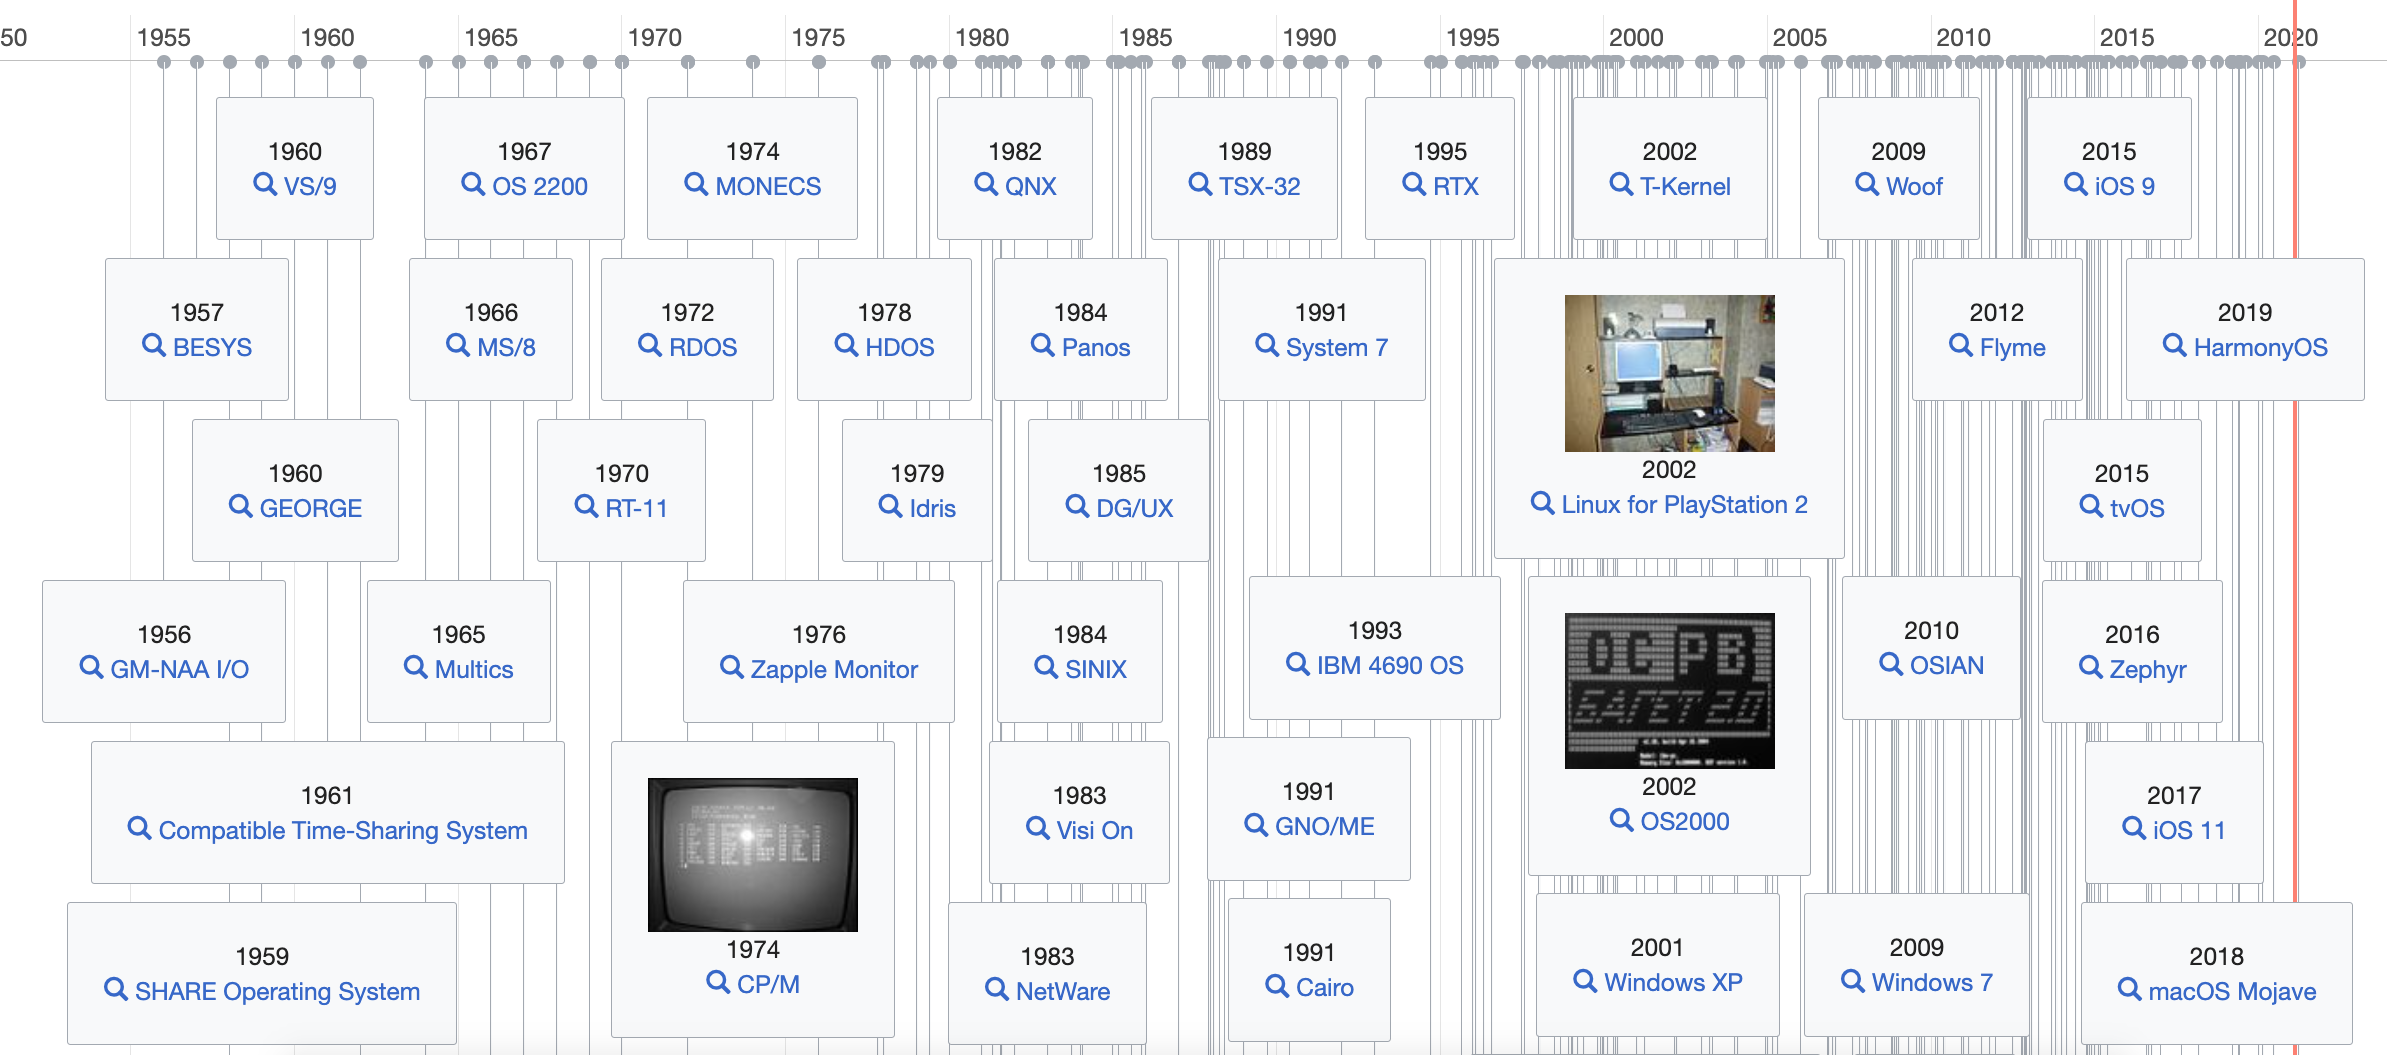
\includegraphics{./chapter/operating_system/os-creation.png}
	\caption{Часть временной шкалы с датами выпуска операционных систем с 1955 по 2020 год.}
	\label{fig:os_creation}
\end{figure*}

\section{Количество операционных систем, написанных на языках программирования}
В листинге \ref{lst:count_os_on_languages} представлен SPARQL-запрос для получения списка языков программирования с выводом количества написанных на них ОС.

\footnotetext{Создание операционной системы длительный процесс, часто занимающий годы. В данном случае указывается дата когда системы была предоставлена в открытый доступ}

\index{SPARQL!COUNT!Языки программирования и число операционных систем}
\begin{lstlisting}[ language=SPARQL, 
	caption={\href{https://w.wiki/uat}{Список языков программирования и количество написанных на них операционных систем}\protect\footnotemark},
	label=lst:count_os_on_languages
	]
# Languages and number of OS written in these languages
SELECT ?lang ?langLabel (COUNT(*) AS ?countOS)
WHERE 
{
	?os wdt:P31 wd:Q9135. # is instance of operating system
	?os wdt:P277 ?lang. # is written in programming language ?lang
SERVICE wikibase:label {bd:serviceParam wikibase:language "ru, en"}
}
GROUP BY ?lang ?langLabel
ORDER BY DESC(?countOS) ASC(?langLabel)
\end{lstlisting}
\footnotetext{Получено \num{24} языков программирования с количеством написанных на них операционных систем в 2017 году и \num{36} в 2021 году. Ссылка на SPARQL-запрос: \href{https://w.wiki/uat}{https://w.wiki/uat}}

Команда ORDER BY DESC(?countOS) ASC(?langLabel) в SPARQL-запросе \ref{lst:count_os_on_languages} используется для двойной сортировки значений в таблице. Все языки программирования будут отсортированы в порядке убывания количества опреционных систем, написанных на них, а при равном их количестве будут отсортированы в алфавитном порядке по названию.

Результат SPARQL-запроса \ref{lst:count_os_on_languages} показывает, что преимущественно ОС пишут на языках си (46 операционных систем) и ассемблер (42 операционные системы). На третьем месте разместился и C++ (16 операционных систем).

С помощью SPARQL-запроса \ref{lst:lang_tree} можно получить диаграмму языков программирования и написанных на них операционных систем в виде дерева (рис.  \ref{fig:prog_lang_os})

\begin{marginfigure}[0.0cm]
	{
		\setlength{\fboxsep}{0pt}%
		\setlength{\fboxrule}{1pt}%
		\fcolorbox{gray}{gray}{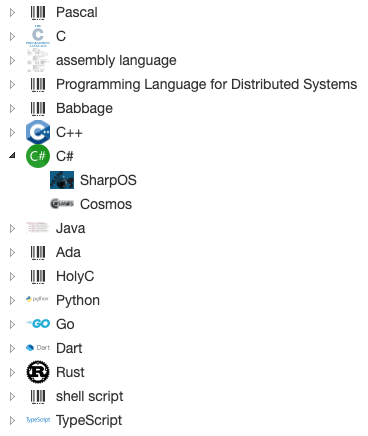
\includegraphics{chapter/operating_system/prog_lang_os.png}}
	}
	\caption{Дерево языков программирования и написанных на них операционных систем}
	\label{fig:prog_lang_os}%
\end{marginfigure}

\marginnote[0.5cm]{
	Сложное задание для самостоятельной работы. Измените скрипт  \ref{lst:lang_tree} (\href{https://w.wiki/ucB}{https://w.wiki/ucB}) так, чтобы рядом с языком программирования было написано число операционных систем,написанных на этом языке.
}

\marginnote[0.5cm]{
	Простое задание для самостоятельной работы. <<Переверните>> скрипт  \ref{lst:lang_tree} (\href{https://w.wiki/ucB}{https://w.wiki/ucB}), то есть строчки верхнего уровня пусть содержат не языки программирования, а операционные системы. При <<разворачивании>> мы должны видеть список языков, на которых написана система.
}

\index{SPARQL!OPTIONAL!Список языков программирования и написанных на них операционных систем}
\index{График!Tree!Дерево языков программирования и написанных на них операционных систем}
\begin{lstlisting}[ language=SPARQL, 
	caption={\href{https://w.wiki/ucB}{Список языков программирования и написанных на них операционных систем}\protect\footnotemark},
	label=lst:lang_tree
	]
# Languages and operating systems written in these languages
#defaultView:Tree
SELECT ?lang ?image ?logoImage ?langLabel 
?os ?osImage ?osLogoImage ?osLabel 
WHERE 
{
	?os wdt:P31 wd:Q9135. # is instance of operating system
	?os wdt:P277 ?lang. # is written in programming language ?lang
	OPTIONAL { ?lang wdt:P18 ?image. }
	OPTIONAL { ?lang wdt:P154 ?logoImage. }
	OPTIONAL { ?os wdt:P18 ?osImage. }
	OPTIONAL { ?os wdt:P154 ?osLogoImage. }
SERVICE wikibase:label {bd:serviceParam wikibase:language "ru, en"}
}
\end{lstlisting}
\footnotetext{Получено \num{146} языков программирования с написанными на них операционными системами в 2021 году. Ссылка на SPARQL-запрос: \href{https://w.wiki/ucB}{https://w.wiki/ucB}}

В этом дереве (рис. \ref{fig:prog_lang_os}) каждая строчка -- это язык программирования. По щелчку мыши можно развернуть язык и увидеть список операционных систем, написанных с использованием этого языка. Если язык или система имеют рисунок или логотип в Викиданных, то они используются в качестве иконок.

\section{Полнота данных}
По данным сайта www.operating-system.org существует 613 операционных систем\cite{list_operating_systems}. В то время как Викиданные на 2017 год содержали информацию лишь о 510 операционных системах (не учитывая \num{667} дистрибутивов Linux\cite{list_operating_systems}). И если просмотреть большое количество объектов в результатах запросов (листинги \ref{lst:inception_time_of_operating_systems} и \ref{lst:count_os_on_languages}), то станет видно, что многие объекты плохо заполнены, а то и вовсе практически пусты (например у систем \wdqName{Novell DOS}{3345389} и \wdqName{MagiC}{1884068} заполнено всего одно свойство\cite{prowd_os_link}.).

В 2020 году Викиданные содержали информацию о 1086 операционных системах (листинг \ref{lst:all_operating_systems}), что свидетельствует о значительных изменениях, а именно за три года (с 2017) количество операционных систем более чем удвоилось с 510 до 1086. Однако большое количество объектов по-прежнему плохо заполнены, например, по результатам запроса \ref{lst:inception_time_of_operating_systems} информация о дате выпуска заполнена всего у \num{238} языков. Из этого можно сделать вывод что Викиданных неполные, но стремительном заполняются.

\section{Языки программирования, используемые для написания операционных систем}
Если взглянуть на количество операционных систем, для которых указано свойство <<язык программирования>>, то можно увидеть что из \num{1086} объектов это свойство заполнено лишь у \num{116}. По данным на 2020 год (рис.~\ref{fig:count-os-written-on-languages}) больше всего операционных систем, а именно 44, написано на языке программирования Cи.

\index{График!BarChart!Количество операционных систем по языкам программирования}
\begin{figure*}[h!]
	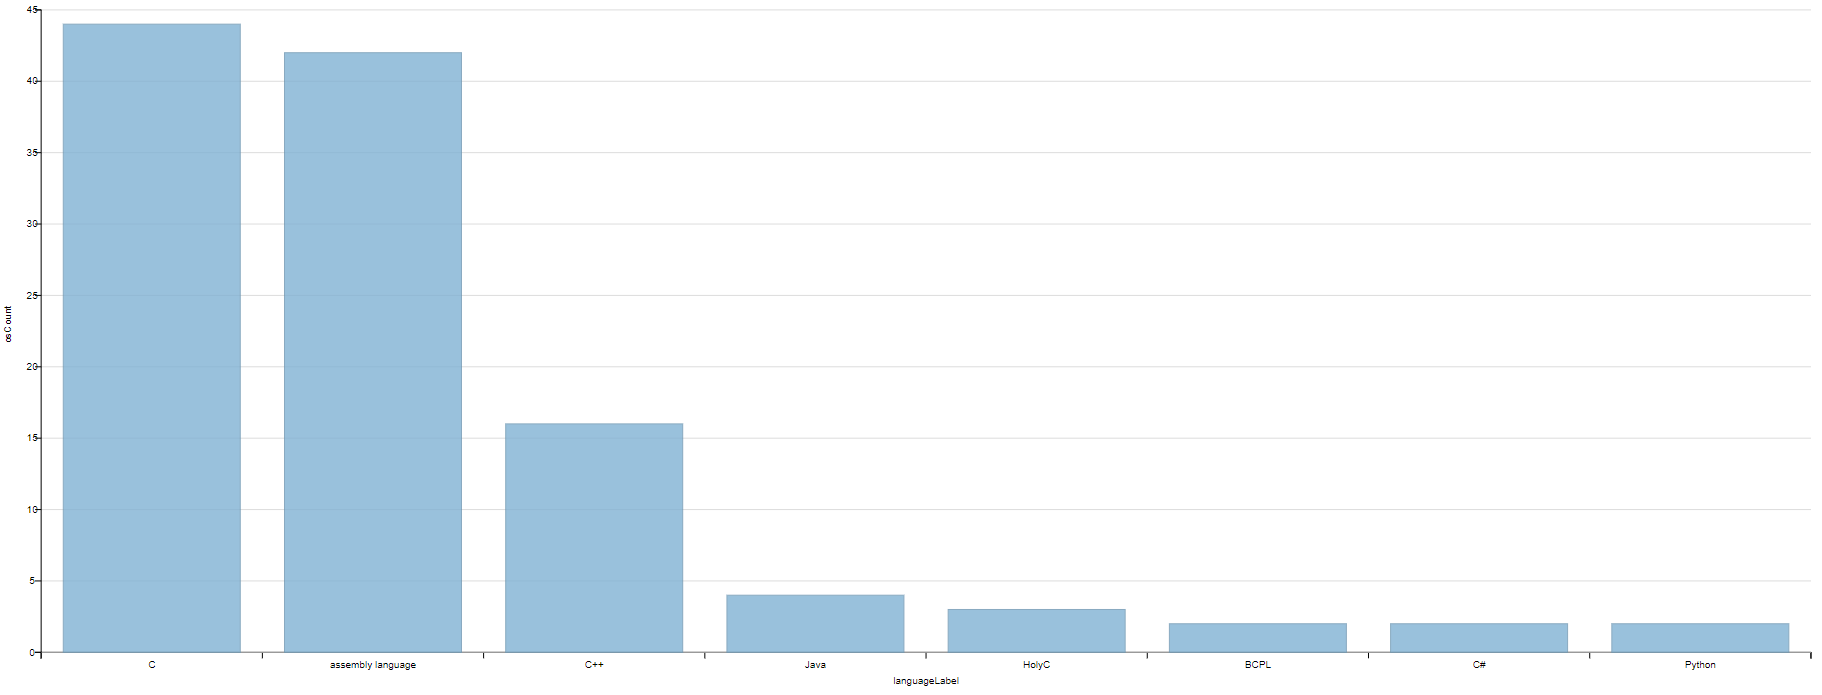
\includegraphics{./chapter/operating_system/count-os-written-on-languages.png}
	\caption{Первые восемь языков, на которых написано больше всего операционных систем, 2020 год}
	\label{fig:count-os-written-on-languages}
\end{figure*}


\section{Количество программ для каждой операционной системы}
В листинге \ref{lst:count_soft_on_os} приведен SPARQL-запрос, показывающий какое количество программ написано для каждой операционной системы.

\index{SPARQL!COUNT!Список операционных систем с количеством программ}
\begin{lstlisting}[ language=SPARQL, 
	caption={\href{https://w.wiki/ugp}{Количество программ для каждой операционной системы}\protect\footnotemark},
	label=lst:count_soft_on_os
	]
# Number of software for each operating system
SELECT ?os ?osLabel (COUNT(*) AS ?softCounter)
WHERE
{ # the software ?soft works on the operating system ?os
	?soft p:P306 [ps:P306 ?os].
SERVICE wikibase:label { bd:serviceParam wikibase:language "ru, en" }
}
GROUP BY ?os ?osLabel
ORDER BY DESC(?softCounter)
\end{lstlisting}
\footnotetext{\num{551} операционная система имела написанные на неё программы в 2020 году. Ссылка на SPARQL-запрос: \href{https://w.wiki/ugp}{https://w.wiki/ugp}}

Лидером среди операционных систем по количеству написанных программ является \wdqName{Linux}{388}, для которого написано \num{9223} программы. Для операционных систем \wdqName{Microsoft Windows}{1406} и  \wdqName{AIX}{269856} (операционной системы производства компании \href{https://www.wikidata.org/wiki/Q37156}{IBM}) создано \num{3278} и \num{2337} программы соответственно.

\section{Сколько компьютерных программ было написано для операционной системы с использованием того или иного языка программирования}
На листинге \ref{lst:count_soft_on_os_with_lang} представлен SPARQL-запрос, показывающий для каждой программы под каждую операционную систему на скольких языках программирования написан компьютерная программа.

\index{SPARQL!COUNT!Список языков программирования с количеством написанного для него программ}
\begin{lstlisting}[ language=SPARQL, 
	caption={\href{https://w.wiki/vDv}{Список операционных систем с количеством программ написанных для них с использованием языков программирования }\protect\footnotemark},
	label=lst:count_soft_on_os_with_lang
	]
#defaultView:BarChart
SELECT ?os ?osLabel (COUNT(*) AS ?softCount)
?softLang ?softLangLabel
WHERE
{
	?soft wdt:P306 ?os. # software works on os
	?soft wdt:P277 ?softLang. # software is written by 
	                          #parogramming language
	?os wdt:P277 ?osLang. # os is written by parogramming language
SERVICE wikibase:label { bd:serviceParam wikibase:language "ru, en"}
}
GROUP BY ?os ?osLabel ?softLang ?softLangLabel
ORDER BY DESC(?count) DESC(?osLabel)
\end{lstlisting}
\footnotetext{ \num{704} компьютерных программ было написано для операционной системы с использованием того или иного языка программирования в 2020 году. Ссылка на SPARQL-запрос: \href{https://w.wiki/vDv}{https://w.wiki/vDv}}

Данный запрос отлично показывает, что большая часть программ, написанных для \href{https://www.wikidata.org/wiki/Q14116}{macOS}, создавалось с использованием \href{https://www.wikidata.org/wiki/Q2407}{C++} (374 программы), \href{https://www.wikidata.org/wiki/Q15777}{Си} (276 программ), \href{https://www.wikidata.org/wiki/Q28865}{Python} (107 программ).
Под \href{https://www.wikidata.org/wiki/Q94}{Android} -- \href{https://www.wikidata.org/wiki/Q2407}{C++} (107 программ) и \href{https://www.wikidata.org/wiki/Q251}{Java} (80 программ).
Под \href{https://www.wikidata.org/wiki/Q48493}{iOS} большинство программ написано на \href{https://www.wikidata.org/wiki/Q2407}{C++} (63 программы).

Гистограмма на рисунке~\ref{fig:count-software-written-on-languages} позволяет увидеть для каждого языка программирования количество программ, которые были на нём написаны, а также под какими ОС работают данные программы. Из графика видно, что наибольшее число программ пишется на языках \href{https://www.wikidata.org/wiki/Q15777}{Си} (2566 программ), \href{https://www.wikidata.org/wiki/Q2407}{C++} (2503 программы), \href{https://www.wikidata.org/wiki/Q251}{Java} (799 программ), \href{https://www.wikidata.org/wiki/Q28865}{Python} (717 программ) и \href{https://www.wikidata.org/wiki/Q2005}{JavaScript} (344 программы).

\begin{figure*}[h!]
	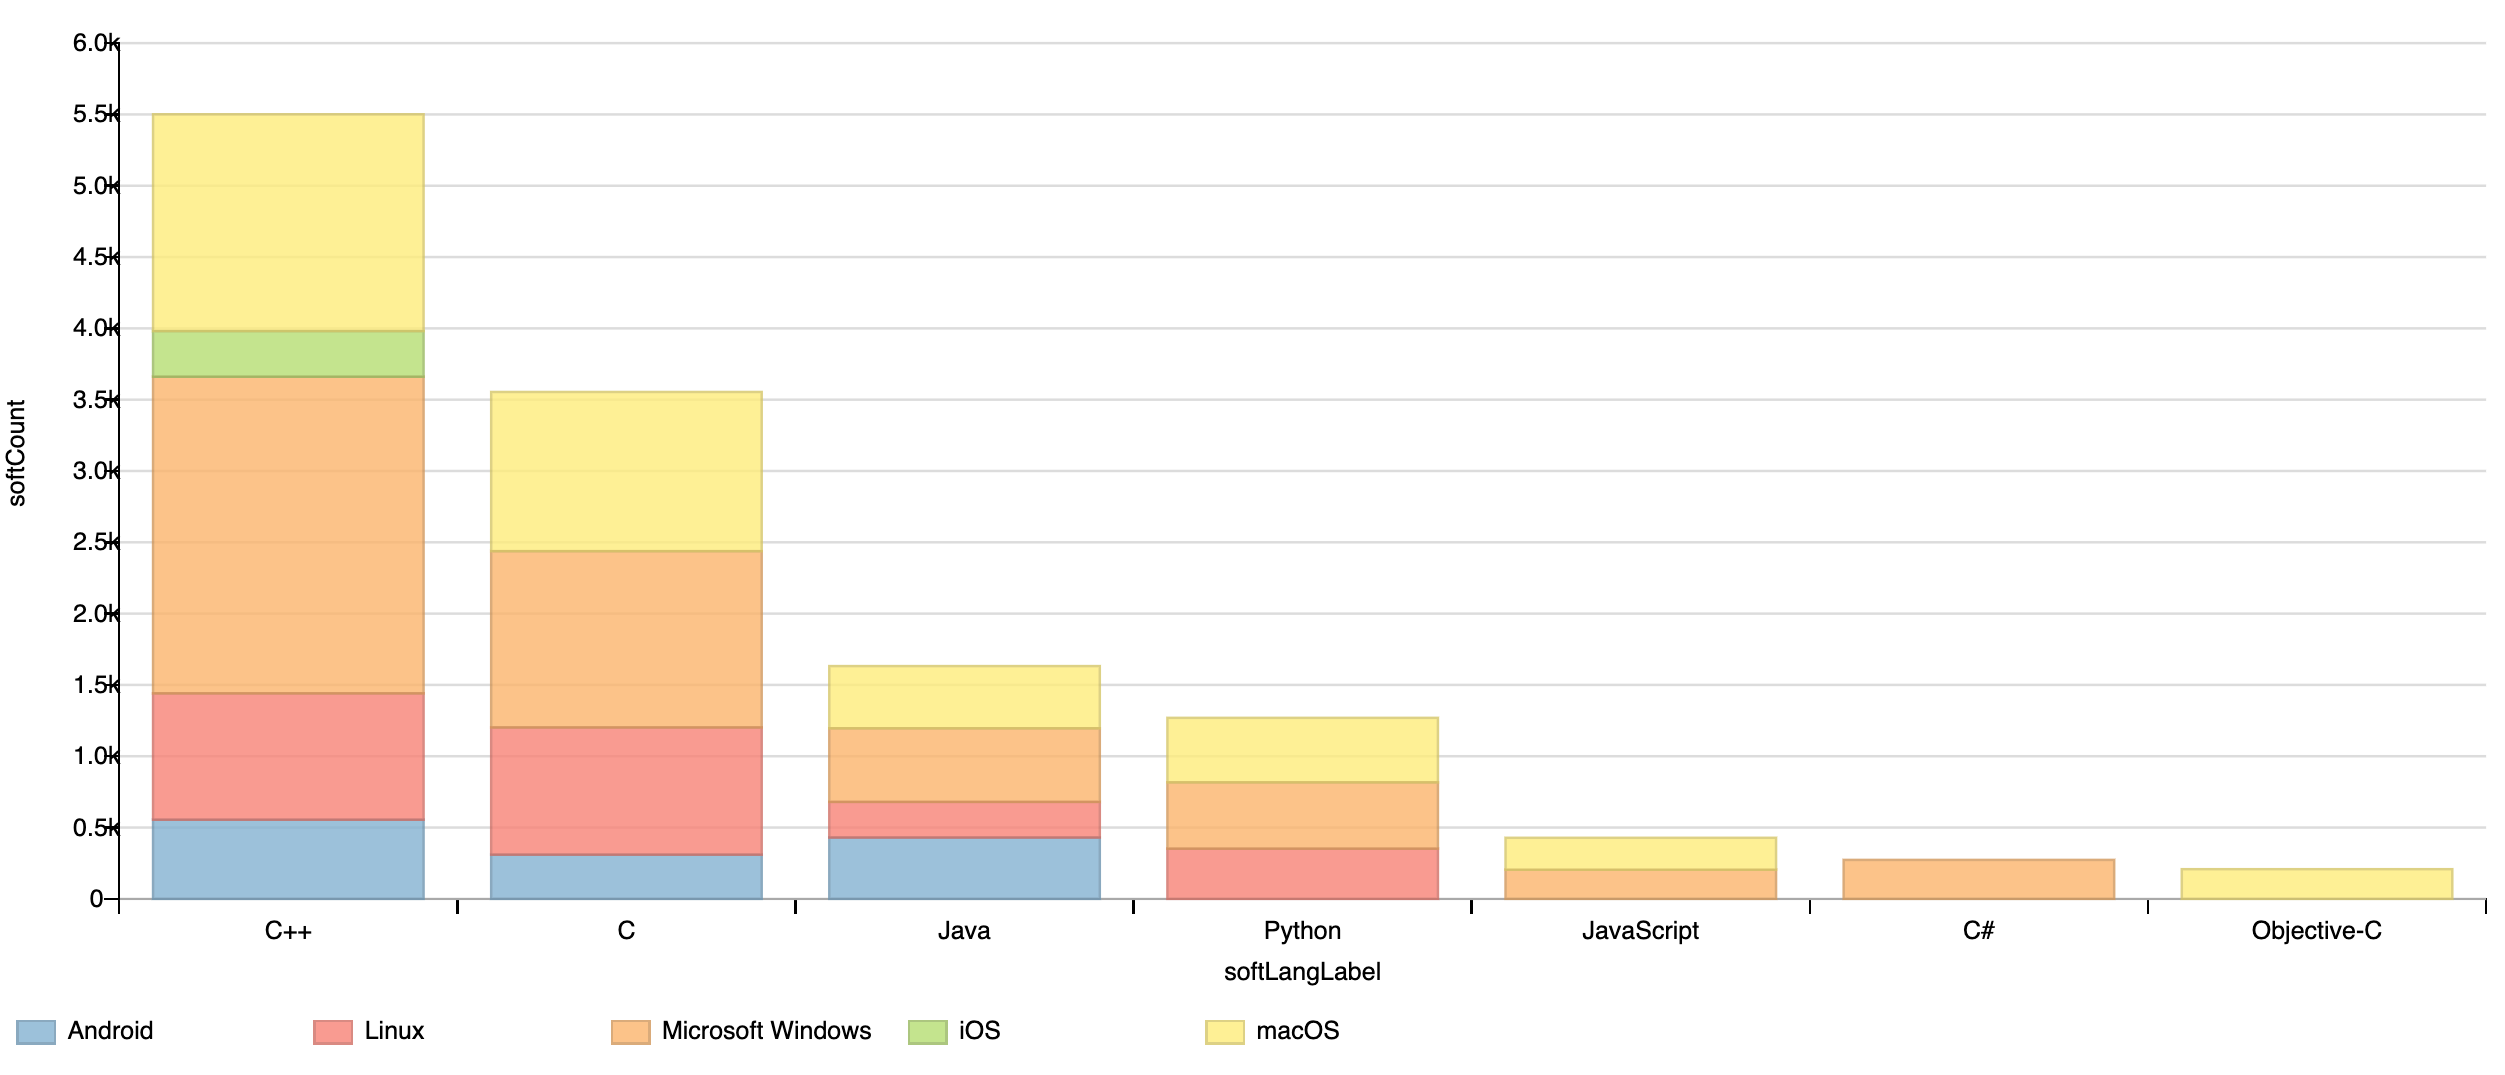
\includegraphics{./chapter/operating_system/Programming-languages-and-count-of-programms-written-on-them-and-OS-2020.png}
	\caption{Языки программирования и количество ОС, под которыми работают программы, написанные на этих языках, 2020 год.}
	\label{fig:count-software-written-on-languages}
\end{figure*}

Рассмотрим каждый из этих языков подробнее.

Большая часть программ на языке С++ пишется под Windows (472 программы) и macOs (300 программ). Несмотря на то что язык С++ был разработан в 1972, он пока не теряет своей популярности за счёт, вероятно, того, что используется для написания низкоуровневых приложений, так как по <<близости>> к аппаратному уровню уступает, разве что, ассемблеру.

Большая часть программ на языке С++ пишется под Windows (700 программ), macOS (400 программ) и Linux (400 программ). Вероятно, С++ будет лидировать ещё долгое время, так как на текущий момент он используется для решений, требующих высокой производительности, чего не позволяют высокоуровневый язык, как Java\cite{lang_performance}.

Большая часть программ на языке Java пишется под macOS (196 программ) и Андроид (156 программ). Вероятно, Java пользуется популярностью за счёт переносимости кода\footnotemark, \footnotetext{Переносимость -- возможность запускать код на множестве платформ без каких-либо изменений.}
то есть код на языке Java запустится на любой машине с установленной JVM\footnotemark.
\marginnote[0.3cm]{}
\footnotetext{Java virtual machine (JVM) --- среда выполнения, которая может выполнять байт-код, полученный в результате компиляции компьютерных программ, написанных на языке программирования Java.}
Большая часть программ на языке JavaScript пишется под macOS (100 программ), Андроид (60 программ) и iOS (40 программ). Как правило, язык используется для написания клиентской части веб-приложений.

Большая часть программ на языке Python пишется под macOS (212 программ) и Linux (107 программ). Язык используется, например, для написания веб-приложений и анализа данных.

Глядя на гистограмму (рис. \ref{fig:count-software-written-on-languages}), можно сделать вывод, что каждый из рассмотренных языков занял свою <<нишу>> в области разработки программ и применяется для определённого круга задач. Отметим, что большая часть ПО пишется под macOS (900 программ), Windows (1500 программ), Linux (1200 программ) или Андроид (300 программ), как это можно увидеть в результате скрипта \ref{lst:count_soft_on_os}.

\section{Документирование ПО}
Викиданные играют большую роль в документировании программного обеспечения. Это показано на примере программ, входящих в среды GNOME и KDE\cite{documenting_wiki}. В этой статье показано, что если в Английской Википедии описаны почти все программы, входящие в состав GNOME и KDE, то в итальянской и французской есть только часть статей. Документирование больших проектов — это известная и трудная задача. Для её решения нужна централизованная система. Именно в этой роли и выступает связка Википедия и Викиданные\cite{documenting_wiki}.

\section{Упражнения}
\label{tasks:operating_system_tasks}
\begin{enumerate}
	\item Вывести список операционных систем с информацией о их разработчиках. Ответ можно найти на странице~\pageref{answer:os_and_developers}.
	\item Вывести список операционных систем с их логотипами. Ответ можно найти на странице~\pageref{answer:os_and_logos}.
	\item Найти страны происхождения операционных систем. Ответ можно найти на странице~\pageref{answer:os_country}.
	\item Создать скрипт создающий диаграмму в виде дерева. Строчки верхнего уровня должны содержать операционные системы. При <<разворачивании>> мы должны видеть список операционных систем, которые основывались на системе из строчки верхнего уровня. Ответ можно найти на странице~\pageref{answer:os_and_bases}.
\end{enumerate}